\documentclass{report}

\usepackage{subfigure}
\usepackage{verbatim}
\usepackage{amsfonts}
\usepackage{amsmath}
\usepackage{tikz}
\usepackage{amsthm}
\usetikzlibrary{shapes}
\usepackage[Conny]{fncychap} % Fancy Chapter headings
\usepackage[english]{babel} % English blind-text
\usepackage{tkz-berge}


\pagestyle{empty}

\tikzstyle{vertex}=[circle,fill=black!25,minimum size=10pt,inner sep=2pt]
\tikzstyle{Nvertex}=[circle,fill=white!25,minimum size=10pt,inner sep=2pt]
\tikzstyle{LabelStyle}=[fill=white,sloped]
\newcommand{\vertexshiftamount}{2.5}
\newcommand{\chem}[1]{\ensuremath{\mathrm{#1}}} % Chemical formula


\newcommand{\tikzpicscale}{1.5}

\newcommand{\TIKZthreeladderA}{
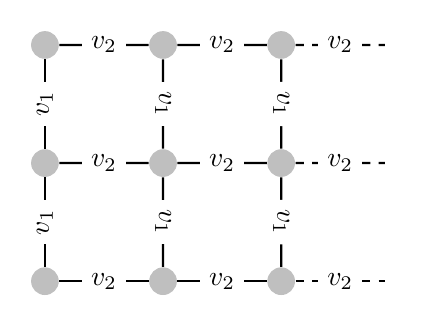
\begin{tikzpicture}[scale=\tikzpicscale]
    \node[vertex] (00) at (0,0)   {};
    \node[vertex] (10) at (1,0)   {};
	 \node[vertex] (20) at (2,0)   {};
    \node[vertex] (01) at (0,1)   {};
    \node[vertex] (11) at (1,1)   {};
    \node[vertex] (21) at (2,1)   {};
    \node[vertex] (02) at (0,2)   {};
    \node[vertex] (12) at (1,2)   {};
    \node[vertex] (22) at (2,2)   {};
	 \Edge[label=$v_2$](00)(10)
	 \Edge[label=$v_2$](10)(20)
	 \Edge[label=$v_2$](01)(11)
	 \Edge[label=$v_2$](11)(21)
	 \Edge[label=$v_2$](02)(12)
	 \Edge[label=$v_2$](12)(22)	
	 \Edge[label=$v_1$](00)(01)
	 \Edge[label=$v_1$](10)(11)
	 \Edge[label=$v_1$](20)(21)
 	 \Edge[label=$v_1$](21)(22)
 	 \Edge[label=$v_1$](11)(12)
 	 \Edge[label=$v_1$](01)(02)
    \node[Nvertex] (n30) at (3,0)   {};
    \node[Nvertex] (n31) at (3,1)   {};
    \node[Nvertex] (n32) at (3,2)   {};
	 \tikzstyle{EdgeStyle}=[dashed]
	 \Edge[label=$v_2$](20)(n30)
	 \Edge[label=$v_2$](21)(n31)
 	 \Edge[label=$v_2$](22)(n32)
\end{tikzpicture}
}

\newcommand{\TIKZthreeladderB}{
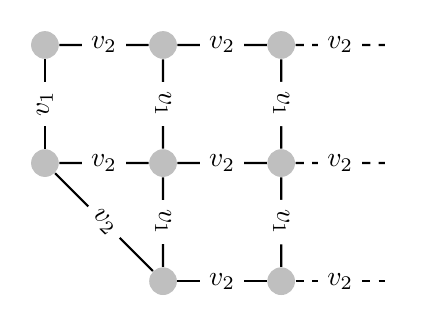
\begin{tikzpicture}[scale=\tikzpicscale]
%    \node[vertex] (00) at (0,0)   {};
    \node[vertex] (10) at (1,0)   {};
	 \node[vertex] (20) at (2,0)   {};
    \node[vertex] (01) at (0,1)   {};
    \node[vertex] (11) at (1,1)   {};
    \node[vertex] (21) at (2,1)   {};
    \node[vertex] (02) at (0,2)   {};
    \node[vertex] (12) at (1,2)   {};
    \node[vertex] (22) at (2,2)   {};
	 \Edge[label=$v_2$](01)(10)
	 \Edge[label=$v_2$](10)(20)
	 \Edge[label=$v_2$](01)(11)
	 \Edge[label=$v_2$](11)(21)
	 \Edge[label=$v_2$](02)(12)
	 \Edge[label=$v_2$](12)(22)	
%)	 \Edge[label=$v_1$](00)(01)
	 \Edge[label=$v_1$](10)(11)
	 \Edge[label=$v_1$](20)(21)
 	 \Edge[label=$v_1$](21)(22)
 	 \Edge[label=$v_1$](11)(12)
 	 \Edge[label=$v_1$](01)(02)
    \node[Nvertex] (n30) at (3,0)   {};
    \node[Nvertex] (n31) at (3,1)   {};
    \node[Nvertex] (n32) at (3,2)   {};
	 \tikzstyle{EdgeStyle}=[dashed]
	 \Edge[label=$v_2$](20)(n30)
	 \Edge[label=$v_2$](21)(n31)
 	 \Edge[label=$v_2$](22)(n32)
\end{tikzpicture}
}

\newcommand{\TIKZthreeladderC}{
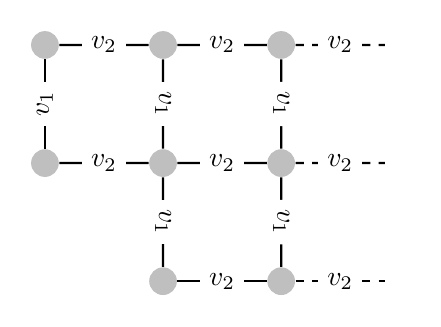
\begin{tikzpicture}[scale=\tikzpicscale]
%    \node[vertex] (00) at (0,0)   {};
    \node[vertex] (10) at (1,0)   {};
	 \node[vertex] (20) at (2,0)   {};
    \node[vertex] (01) at (0,1)   {};
    \node[vertex] (11) at (1,1)   {};
    \node[vertex] (21) at (2,1)   {};
    \node[vertex] (02) at (0,2)   {};
    \node[vertex] (12) at (1,2)   {};
    \node[vertex] (22) at (2,2)   {};
%	 \Edge[label=$v_2$](01)(10)
	 \Edge[label=$v_2$](10)(20)
	 \Edge[label=$v_2$](01)(11)
	 \Edge[label=$v_2$](11)(21)
	 \Edge[label=$v_2$](02)(12)
	 \Edge[label=$v_2$](12)(22)	
%)	 \Edge[label=$v_1$](00)(01)
	 \Edge[label=$v_1$](10)(11)
	 \Edge[label=$v_1$](20)(21)
 	 \Edge[label=$v_1$](21)(22)
 	 \Edge[label=$v_1$](11)(12)
 	 \Edge[label=$v_1$](01)(02)
    \node[Nvertex] (n30) at (3,0)   {};
    \node[Nvertex] (n31) at (3,1)   {};
    \node[Nvertex] (n32) at (3,2)   {};
	 \tikzstyle{EdgeStyle}=[dashed]
	 \Edge[label=$v_2$](20)(n30)
	 \Edge[label=$v_2$](21)(n31)
 	 \Edge[label=$v_2$](22)(n32)
\end{tikzpicture}
}

\newcommand{\TIKZthreeladderD}{
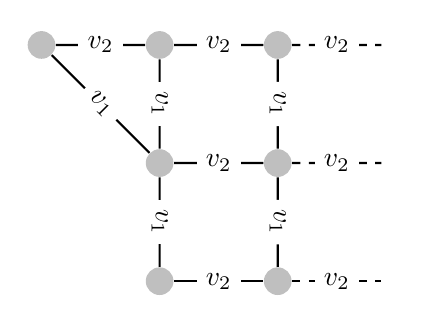
\begin{tikzpicture}[scale=\tikzpicscale]
%    \node[vertex] (00) at (0,0)   {};
    \node[vertex] (10) at (1,0)   {};
	 \node[vertex] (20) at (2,0)   {};
%    \node[vertex] (01) at (0,1)   {};
    \node[vertex] (11) at (1,1)   {};
    \node[vertex] (21) at (2,1)   {};
    \node[vertex] (02) at (0,2)   {};
    \node[vertex] (12) at (1,2)   {};
    \node[vertex] (22) at (2,2)   {};
%	 \Edge[label=$v_2$](01)(10)
	 \Edge[label=$v_2$](10)(20)
%	 \Edge[label=$v_2$](01)(11)
	 \Edge[label=$v_2$](11)(21)
	 \Edge[label=$v_2$](02)(12)
	 \Edge[label=$v_2$](12)(22)	
%)	 \Edge[label=$v_1$](00)(01)
	 \Edge[label=$v_1$](10)(11)
	 \Edge[label=$v_1$](20)(21)
 	 \Edge[label=$v_1$](21)(22)
 	 \Edge[label=$v_1$](11)(12)
 	 \Edge[label=$v_1$](11)(02)
    \node[Nvertex] (n30) at (3,0)   {};
    \node[Nvertex] (n31) at (3,1)   {};
    \node[Nvertex] (n32) at (3,2)   {};
	 \tikzstyle{EdgeStyle}=[dashed]
	 \Edge[label=$v_2$](20)(n30)
	 \Edge[label=$v_2$](21)(n31)
 	 \Edge[label=$v_2$](22)(n32)
\end{tikzpicture}
}

\newcommand{\TIKZthreeladderE}{
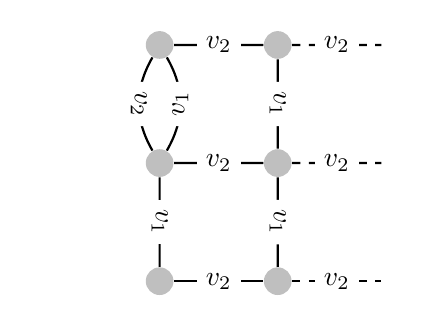
\begin{tikzpicture}[scale=\tikzpicscale]
    \node[Nvertex] (00) at (0,0)   {};
    \node[vertex] (10) at (1,0)   {};
	 \node[vertex] (20) at (2,0)   {};
%    \node[vertex] (01) at (0,1)   {};
    \node[vertex] (11) at (1,1)   {};
    \node[vertex] (21) at (2,1)   {};
%    \node[vertex] (02) at (0,2)   {};
    \node[vertex] (12) at (1,2)   {};
    \node[vertex] (22) at (2,2)   {};
%	 \Edge[label=$v_2$](01)(10)
	 \Edge[label=$v_2$](10)(20)
%	 \Edge[label=$v_2$](01)(11)
	 \Edge[label=$v_2$](11)(21)
%	 \Edge[label=$v_2$](02)(12)
	 \Edge[label=$v_2$](12)(22)	
%)	 \Edge[label=$v_1$](00)(01)
	 \Edge[label=$v_1$](10)(11)
	 \Edge[label=$v_1$](20)(21)
 	 \Edge[label=$v_1$](21)(22)
% 	 \Edge[label=$v_1$](11)(02)
    \node[Nvertex] (n30) at (3,0)   {};
    \node[Nvertex] (n31) at (3,1)   {};
    \node[Nvertex] (n32) at (3,2)   {};
	 \tikzstyle{EdgeStyle}=[dashed]
	 \Edge[label=$v_2$](20)(n30)
	 \Edge[label=$v_2$](21)(n31)
 	 \Edge[label=$v_2$](22)(n32)
 	 \tikzstyle{EdgeStyle}=[bend left]
  	 \Edge[label=$v_2$](11)(12)
  	 \tikzstyle{EdgeStyle}=[bend right]
  	 \Edge[label=$v_1$](11)(12)
\end{tikzpicture}
}

\newcommand{\TIKZthreeladderF}{
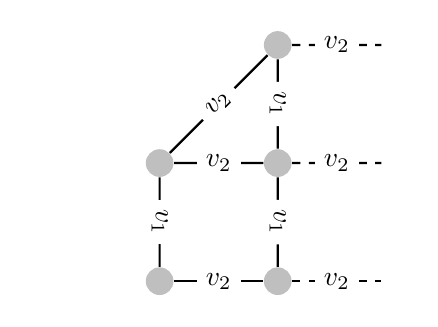
\begin{tikzpicture}[scale=\tikzpicscale]
    \node[Nvertex] (00) at (0,0)   {};
    \node[vertex] (10) at (1,0)   {};
	 \node[vertex] (20) at (2,0)   {};
%    \node[vertex] (01) at (0,1)   {};
    \node[vertex] (11) at (1,1)   {};
    \node[vertex] (21) at (2,1)   {};
%    \node[vertex] (02) at (0,2)   {};
%    \node[vertex] (12) at (1,2)   {};
    \node[vertex] (22) at (2,2)   {};
%	 \Edge[label=$v_2$](01)(10)
	 \Edge[label=$v_2$](10)(20)
%	 \Edge[label=$v_2$](01)(11)
	 \Edge[label=$v_2$](11)(21)
%	 \Edge[label=$v_2$](02)(12)
	 \Edge[label=$v_2$](11)(22)	
%)	 \Edge[label=$v_1$](00)(01)
	 \Edge[label=$v_1$](10)(11)
	 \Edge[label=$v_1$](20)(21)
 	 \Edge[label=$v_1$](21)(22)
% 	 \Edge[label=$v_1$](11)(02)
    \node[Nvertex] (n30) at (3,0)   {};
    \node[Nvertex] (n31) at (3,1)   {};
    \node[Nvertex] (n32) at (3,2)   {};
	 \tikzstyle{EdgeStyle}=[dashed]
	 \Edge[label=$v_2$](20)(n30)
	 \Edge[label=$v_2$](21)(n31)
 	 \Edge[label=$v_2$](22)(n32)
  	 %\tikzstyle{EdgeStyle}=[loop above]
  	 %\Edge[label=$v_1$](11)(11)
\end{tikzpicture}
}

\newcommand{\TIKZthreeladderG}{
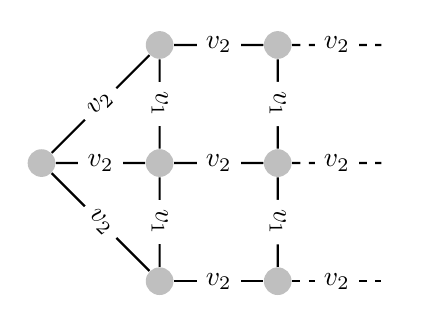
\begin{tikzpicture}[scale=\tikzpicscale]
%    \node[vertex] (00) at (0,0)   {};
    \node[vertex] (10) at (1,0)   {};
	 \node[vertex] (20) at (2,0)   {};
    \node[vertex] (01) at (0,1)   {};
    \node[vertex] (11) at (1,1)   {};
    \node[vertex] (21) at (2,1)   {};
%    \node[vertex] (02) at (0,2)   {};
    \node[vertex] (12) at (1,2)   {};
    \node[vertex] (22) at (2,2)   {};
	 \Edge[label=$v_2$](01)(10)
	 \Edge[label=$v_2$](10)(20)
	 \Edge[label=$v_2$](01)(11)
	 \Edge[label=$v_2$](11)(21)
	 \Edge[label=$v_2$](01)(12)
	 \Edge[label=$v_2$](12)(22)	
%)	 \Edge[label=$v_1$](00)(01)
	 \Edge[label=$v_1$](10)(11)
	 \Edge[label=$v_1$](20)(21)
 	 \Edge[label=$v_1$](21)(22)
 	 \Edge[label=$v_1$](11)(12)
% 	 \Edge[label=$v_1$](01)(02)
    \node[Nvertex] (n30) at (3,0)   {};
    \node[Nvertex] (n31) at (3,1)   {};
    \node[Nvertex] (n32) at (3,2)   {};
	 \tikzstyle{EdgeStyle}=[dashed]
	 \Edge[label=$v_2$](20)(n30)
	 \Edge[label=$v_2$](21)(n31)
 	 \Edge[label=$v_2$](22)(n32)
\end{tikzpicture}
}

\newcommand{\TIKZthreeladderH}{
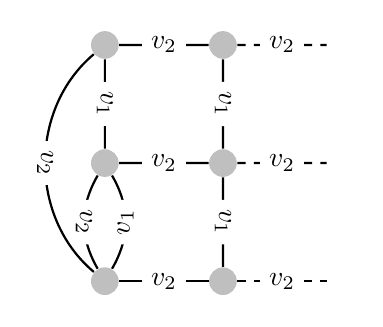
\begin{tikzpicture}[scale=\tikzpicscale]
%    \node[vertex] (00) at (0,0)   {};
    \node[vertex] (10) at (1,0)   {};
	 \node[vertex] (20) at (2,0)   {};
%    \node[vertex] (01) at (0,1)   {};
    \node[vertex] (11) at (1,1)   {};
    \node[vertex] (21) at (2,1)   {};
%    \node[vertex] (02) at (0,2)   {};
    \node[vertex] (12) at (1,2)   {};
    \node[vertex] (22) at (2,2)   {};
	 \Edge[label=$v_2$](10)(20)
%	 \Edge[label=$v_2$](01)(11)
	 \Edge[label=$v_2$](11)(21)
%	 \Edge[label=$v_2$](01)(12)
	 \Edge[label=$v_2$](12)(22)	
%)	 \Edge[label=$v_1$](00)(01)
	 \Edge[label=$v_1$](20)(21)
 	 \Edge[label=$v_1$](21)(22)
 	 \Edge[label=$v_1$](11)(12)
% 	 \Edge[label=$v_1$](01)(02)
    \node[Nvertex] (n30) at (3,0)   {};
    \node[Nvertex] (n31) at (3,1)   {};
    \node[Nvertex] (n32) at (3,2)   {};
	 \tikzstyle{EdgeStyle}=[dashed]
	 \Edge[label=$v_2$](20)(n30)
	 \Edge[label=$v_2$](21)(n31)
 	 \Edge[label=$v_2$](22)(n32)
 	 
 	 \tikzstyle{EdgeStyle}=[bend left]
 	 \Edge[label=$v_2$](10)(11)
  	 \tikzstyle{EdgeStyle}=[bend left=50]
 	 \Edge[label=$v_2$](10)(12)
  	 %\Edge[label=$v_2$](11)(12)
 	 \tikzstyle{EdgeStyle}=[bend right]
	 \Edge[label=$v_1$](10)(11)
\end{tikzpicture}
}

\newcommand{\TIKZthreeladderI}{
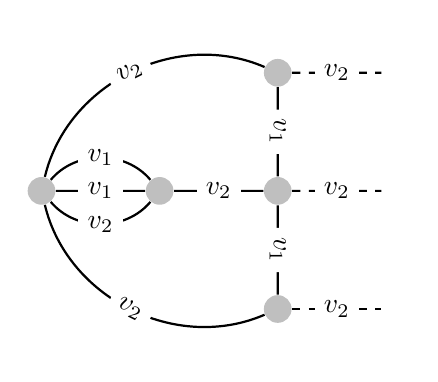
\begin{tikzpicture}[scale=\tikzpicscale]
%    \node[vertex] (00) at (0,0)   {};
%    \node[vertex] (10) at (1,0)   {};
	 \node[vertex] (20) at (2,0)   {};
    \node[vertex] (01) at (0,1)   {};
    \node[vertex] (11) at (1,1)   {};
    \node[vertex] (21) at (2,1)   {};
%    \node[vertex] (02) at (0,2)   {};
%    \node[vertex] (12) at (1,2)   {};
    \node[vertex] (22) at (2,2)   {};
%	 \Edge[label=$v_2$](01)(10)
%	 \Edge[label=$v_2$](10)(20)
%	 \Edge[label=$v_2$](01)(21)
	 \Edge[label=$v_2$](11)(21)
%	 \Edge[label=$v_2$](12)(22)	
%)	 \Edge[label=$v_1$](00)(01)
%	 \Edge[label=$v_1$](10)(11)
	 \Edge[label=$v_1$](20)(21)
 	 \Edge[label=$v_1$](21)(22)
% 	 \Edge[label=$v_1$](11)(12)
% 	 \Edge[label=$v_1$](01)(02)
    \node[Nvertex] (n30) at (3,0)   {};
    \node[Nvertex] (n31) at (3,1)   {};
    \node[Nvertex] (n32) at (3,2)   {};
	 \tikzstyle{EdgeStyle}=[dashed]
	 \Edge[label=$v_2$](20)(n30)
	 \Edge[label=$v_2$](21)(n31)
 	 \Edge[label=$v_2$](22)(n32)

	 \tikzstyle{EdgeStyle}=[]
	 \Edge[label=$v_1$](01)(11)
  	 \tikzstyle{EdgeStyle}=[bend left=50]
	 \Edge[label=$v_2$](01)(22)
 	 \Edge[label=$v_1$](01)(11)
  	 \tikzstyle{EdgeStyle}=[bend right=50]
 	 \Edge[label=$v_2$](01)(20)
 	 \Edge[label=$v_2$](01)(11)
\end{tikzpicture}
}


\newcommand{\TIKZthreeladderJ}{
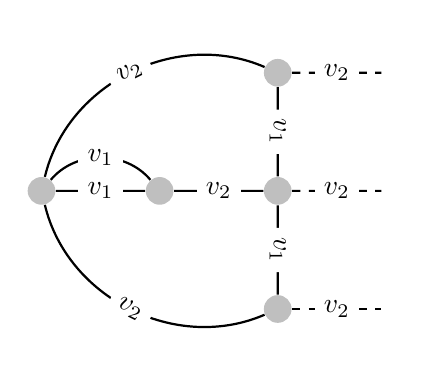
\begin{tikzpicture}[scale=\tikzpicscale]
%    \node[vertex] (00) at (0,0)   {};
%    \node[vertex] (10) at (1,0)   {};
	 \node[vertex] (20) at (2,0)   {};
    \node[vertex] (01) at (0,1)   {};
    \node[vertex] (11) at (1,1)   {};
    \node[vertex] (21) at (2,1)   {};
%    \node[vertex] (02) at (0,2)   {};
%    \node[vertex] (12) at (1,2)   {};
    \node[vertex] (22) at (2,2)   {};
%	 \Edge[label=$v_2$](01)(10)
%	 \Edge[label=$v_2$](10)(20)
%	 \Edge[label=$v_2$](01)(21)
	 \Edge[label=$v_2$](11)(21)
%	 \Edge[label=$v_2$](12)(22)	
%)	 \Edge[label=$v_1$](00)(01)
%	 \Edge[label=$v_1$](10)(11)
	 \Edge[label=$v_1$](20)(21)
 	 \Edge[label=$v_1$](21)(22)
% 	 \Edge[label=$v_1$](11)(12)
% 	 \Edge[label=$v_1$](01)(02)
    \node[Nvertex] (n30) at (3,0)   {};
    \node[Nvertex] (n31) at (3,1)   {};
    \node[Nvertex] (n32) at (3,2)   {};
	 \tikzstyle{EdgeStyle}=[dashed]
	 \Edge[label=$v_2$](20)(n30)
	 \Edge[label=$v_2$](21)(n31)
 	 \Edge[label=$v_2$](22)(n32)

	 \tikzstyle{EdgeStyle}=[]
	 \Edge[label=$v_1$](01)(11)
  	 \tikzstyle{EdgeStyle}=[bend left=50]
	 \Edge[label=$v_2$](01)(22)
 	 \Edge[label=$v_1$](01)(11)
  	 \tikzstyle{EdgeStyle}=[bend right=50]
 	 \Edge[label=$v_2$](01)(20)
% 	 \Edge[label=$v_2$](01)(11)
\end{tikzpicture}
}


\begin{document}

\tikzstyle{big_vertex}=[circle,fill=red!15,minimum size=50pt,inner sep=2pt,draw=black!50]
\tikzstyle{med_vertex}=[circle,fill=red!10,minimum size=35pt,inner sep=2pt,draw=black!50]



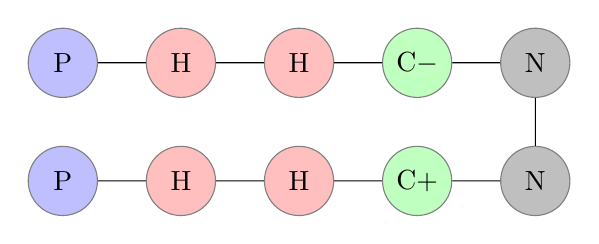
\begin{tikzpicture}[scale=\tikzpicscale]
    \tikzstyle{hvertex}=[circle,fill=red!25,minimum size=25pt,inner sep=2pt,draw=black!50]
    \tikzstyle{pvertex}=[circle,fill=blue!25,minimum size=25pt,inner sep=2pt,draw=black!50]
    \tikzstyle{cpvertex}=[circle,fill=green!25,minimum size=25pt,inner sep=2pt,draw=black!50]
    \tikzstyle{nvertex}=[circle,fill=black!25,minimum size=25pt,inner sep=2pt,draw=black!50]

    \node[pvertex] (r0) at (0,0)   {\chem{P}};
    \node[hvertex] (r1) at (1,0)   {\chem{H}};
    \node[hvertex] (r2) at (2,0)   {\chem{H}};
    \node[cpvertex] (r3) at (3,0)   {\chem{C+}};
    \node[nvertex] (r4) at (4,0)   {\chem{N}};
    \node[nvertex] (r5) at (4,1)   {\chem{N}};
    \node[cpvertex] (r6) at (3,1)   {\chem{C-}};
    \node[hvertex] (r7) at (2,1)   {\chem{H}};
    \node[hvertex] (r8) at (1,1)   {\chem{H}};
    \node[pvertex] (r9) at (0,1)   {\chem{P}};

    \draw [] (r0)--(r1)--(r2)--(r3)--(r4)--(r5)--(r6)--(r7)--(r8)--(r9)--cycle;
   
\end{tikzpicture}

\begin{tikzpicture}[scale=\tikzpicscale]
    \node[vertex] (U) at (0,0)   {$U$};
    \node[med_vertex] (I) at (\vertexshiftamount,0)   {$I$};
    \node[big_vertex] (F) at (2*\vertexshiftamount,.5*\vertexshiftamount)   {$F$};
    \node[big_vertex] (M) at (2*\vertexshiftamount,-.5*\vertexshiftamount)   {$M$};

    \Edge[label=$w_{\chem{U I}}$](U)(I)
    \Edge[label=$w_{\chem{I M}}$](I)(M)
    \Edge[label=$w_{\chem{IF}}$](I)(F)
\end{tikzpicture}

\begin{tikzpicture}[scale=\tikzpicscale]


  \node[big_vertex] (c1) at (0,0)   {$c_1$};
  \node[big_vertex] (c2) at (1*\vertexshiftamount,0)   {$c_2$};
  \node[vertex]    (c3) at (2*\vertexshiftamount,0)   {$c_3$};
  \node[big_vertex] (c0) at (3*\vertexshiftamount,0)   {$c_0$};
  
  \draw [] (c0) -> node[above=.1cm] {$w_{\rightarrow}=3130$} (c3);
  \draw [] (c0) -> node[below=.1cm] {$w_{\leftarrow}=29$} (c3);

  \draw [] (c2) -> node[above=.1cm] {$w_{\leftarrow}=1198$} (c3);  
  \draw [] (c2) -> node[below=.1cm] {$w_{\rightarrow}=4$} (c3);
  
  \draw [] (c2) -- node[below=.1cm] {$w_{\leftarrow}=37$} (c1);
  \draw [] (c2) -- node[above=.1cm] {$w_{\rightarrow}=61$} (c1);
\end{tikzpicture}

\end{document}


\begin{comment}
\hspace{-5em}
\begin{tabular}{ c c c}
$Z(n)$            & $B(n)$               & $C(n)$ \\
\TIKZthreeladderA & \TIKZthreeladderB & \TIKZthreeladderC \\ 
$D(n)$               & $E(n)$               & $F(n)$ \\
\TIKZthreeladderD & \TIKZthreeladderE & \TIKZthreeladderF \\ 
$H(n)$               & $I(n)$               & $J(n)$ \\
\TIKZthreeladderH & \TIKZthreeladderI & \TIKZthreeladderJ \\ 
\end{tabular}
\begin{align}
Z(n) &= v_1 B(n) + (q+v_2) C(n) \\
C(n) &= v_1 D(n) + (q+v_2)^2 Z(n-1) \\
D(n) &= v_1 E(n) + (q+v_2) Z(n-1) \\
E(n) &= v_2(1+v_1) F(n) + Z(n-1) \\
B(n) &= v_1 G(n) + (q+v_2) D(n) \\
G(n) &= v_2 E(n) + (q+v_2)Z(n-1) + v_2 H(n) \\
H(n) &= v_2 I(n) + E(n) \\
I(n) &= v_2 (1+v_1)^2 G(n-1) + J(n) \\
J(n) &= v_1 (1+v_1) G(n-1)  + v_1 G(n-1) \\
     &\hspace{2em} + (v_2 + q)( Z(n-2)(1+ (v_2+q)) J(n-1) ) \\
F(n) &= B(n-1)
\end{align}
\end{comment}


\begin{comment}
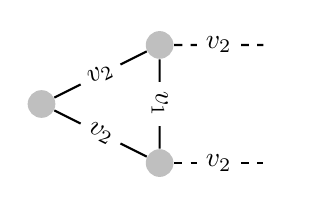
\begin{tikzpicture}[scale=\tikzpicscale]
    \node[vertex] (G2) at (1,0)   {};
    \node[vertex] (GB) at (1,1)   {};
    \node[vertex] (G1A) at (0,.5)   {};
    
	 \Edge[label=$v_2$](G1A)(G2)
	 \Edge[label=$v_2$](G1A)(GB)
	 \Edge[label=$v_1$](G2)(GB)
    \node[Nvertex] (G3) at (2,0)   {};
    \node[Nvertex] (GC) at (2,1)   {};
	 \tikzstyle{EdgeStyle}=[dashed]
	 \Edge[label=$v_2$](G2)(G3)
	 \Edge[label=$v_2$](GB)(GC)
\end{tikzpicture}

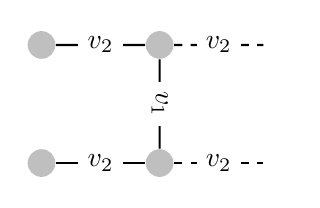
\begin{tikzpicture}[scale=\tikzpicscale]
    \node[vertex] (G1) at (0,0)   {};
    \node[vertex] (G2) at (1,0)   {};
    \node[vertex] (GA) at (0,1)   {};
    \node[vertex] (GB) at (1,1)   {};
	 \Edge[label=$v_2$](G1)(G2)
	 \Edge[label=$v_2$](GA)(GB)
	 %\Edge[label=$v_1$](G1)(GA)
	 \Edge[label=$v_1$](G2)(GB)
    \node[Nvertex] (G3) at (2,0)   {};
    \node[Nvertex] (GC) at (2,1)   {};
	 \tikzstyle{EdgeStyle}=[dashed]
	 \Edge[label=$v_2$](G2)(G3)
	 \Edge[label=$v_2$](GB)(GC)
\end{tikzpicture}

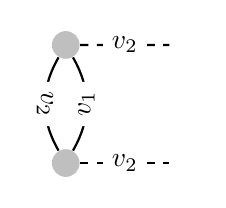
\begin{tikzpicture}[scale=\tikzpicscale]
    \node[vertex] (G2) at (1,0)   {};
    \node[vertex] (GB) at (1,1)   {};

	 %\Edge[label=$v_1$](G1)(GA)
	\tikzstyle{EdgeStyle}=[bend left]
	\Edge[label=$v_2$](G2)(GB)
	
  	\tikzstyle{EdgeStyle}=[bend right]
	\Edge[label=$v_1$](G2)(GB)
	 
    \node[Nvertex] (G3) at (2,0)   {};
    \node[Nvertex] (GC) at (2,1)   {};
	 \tikzstyle{EdgeStyle}=[dashed]
	 \Edge[label=$v_2$](G2)(G3)
	 \Edge[label=$v_2$](GB)(GC)
\end{tikzpicture}

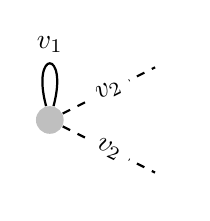
\begin{tikzpicture}[scale=\tikzpicscale]
    \node[vertex] (G2B) at (1,.5)   {};

	 %\Edge[label=$v_1$](G1)(GA)
	\tikzstyle{EdgeStyle}=[loop above]
	\Edge[label=$v_1$](G2B)(G2B)
	
   \node[Nvertex] (G3) at (2,0)   {};
   \node[Nvertex] (GC) at (2,1)   {};
	\tikzstyle{EdgeStyle}=[dashed]
	\Edge[label=$v_2$](G2B)(G3)
	\Edge[label=$v_2$](G2B)(GC)
\end{tikzpicture}


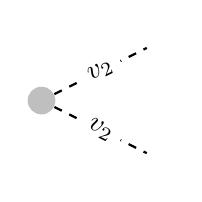
\begin{tikzpicture}[scale=\tikzpicscale]
    \node[vertex] (G2B) at (1,.5)   {};


   \node[Nvertex] (G3) at (2,0)   {};
   \node[Nvertex] (GC) at (2,1)   {};
	\tikzstyle{EdgeStyle}=[dashed]
	\Edge[label=$v_2$](G2B)(G3)
	\Edge[label=$v_2$](G2B)(GC)
\end{tikzpicture}
\end{comment}
